\paragraph{一个\trSpectralSequence。}\label{sub:spectral-sequence}
设 $\boldsymbol{\gamma}$ 是\trVanishingPath{}的一个\trDistinguishedBasis，而 $\boldsymbol{\delta}$ 是对 $\boldsymbol{\gamma}$ 施加相应于 \eqref{eq:global-half-twist} 中元素 $\Delta^{1/2}\in\mathrm{Br}_m$ 的那些\trHurwitz{}移动之后所得的基（注意，虽然这是\trBraidGroup{}中的一个正元素，但\cref{sub:distinguished-bases}中的讨论意味着，在几何上，\trDisk{}的相应\trDiffeomorphism{}是沿一条平行于边界的\trCircle{}的负\trDehnTwist{}的平方根）。此外，我们还想考虑路径的集合 $\boldsymbol{\gamma}^{!}$，它是把基点从 $*$ 出发沿一个顺时针半圆移到 $-*$ 而从 $\boldsymbol{\delta}$ 得到的；参见\cref{fig:basepoint-move-paths}。
\begin{figure}[htbp]
\centering
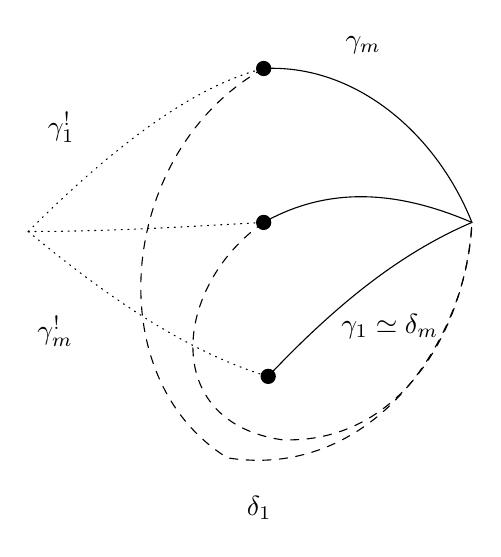
\begin{tikzpicture}[line cap=round,line join=round,scale=1.15]
\fill (2.6,4.0) circle (2.4pt);
\fill (2.6,2.3) circle (2.4pt);
\fill (2.65,0.6) circle (2.4pt);
\draw (2.6,4.0) .. controls (3.6,4.05) and (4.5,3.3) .. (4.9,2.3);
\node[anchor=south] at (3.7,4.05) {$\gamma_m$};
\draw (2.6,2.3) .. controls (3.4,2.75) and (4.2,2.6) .. (4.9,2.3);
\draw (2.65,0.6) .. controls (3.5,1.5) and (4.2,2.0) .. (4.9,2.3);
\node[anchor=west] at (3.35,1.15) {$\gamma_1\simeq\delta_m$};
\draw[dotted] (0,2.2) .. controls (0.9,3.1) and (1.8,3.8) .. (2.6,4.0);
\node[anchor=east] at (0.62,3.35) {$\gamma^{!}_1$};
\draw[dotted] (0,2.2) .. controls (0.9,2.2) and (1.7,2.25) .. (2.6,2.3);
\draw[dotted] (0,2.2) .. controls (0.9,1.45) and (1.8,0.85) .. (2.65,0.6);
\node[anchor=east] at (0.6,1.1) {$\gamma^{!}_m$};
\draw[dashed] (2.6,4.0) .. controls (1.0,3.1) and (0.75,0.6) .. (2.2,-0.3)
      .. controls (3.8,-0.55) and (4.85,1.0) .. (4.9,2.3);
\draw[dashed] (2.6,2.3) .. controls (1.6,1.6) and (1.45,0.1) .. (2.8,-0.1)
      .. controls (4.1,-0.15) and (4.83,1.1) .. (4.9,2.3);
\node[anchor=north] at (2.55,-0.62) {$\delta_1$};
\end{tikzpicture}
\caption{}\label{fig:basepoint-move-paths}
\end{figure}
设 $L^{\#}_j$（$j=0,1$）是含于 $E^{\mathrm{shrink}}$ 之内的两个\trBrane，并令 $\widetilde{L}^{\#}_j$ 为由此所得的 (U) 型\trEquivariant\trBrane。我们将把这两个\trBrane{}看成 $D\scr{F}(\pi)$ 中的\trObject{}来应用\cref{thm:beilinson-spectral-sequence}。结果是一个\trConvergence{}到
\begin{equation*}
HF^{*}(\widetilde{L}^{\#}_0,\widetilde{L}^{\#}_1)^{\ZZ/2}\cong HF^{*}(L^{\#}_0,L^{\#}_1),
\end{equation*}
的\trSpectralSequence，其中该\trIsomorphism{}是\cref{thm:full-embedding-functor}的一部分。这个\trSpectralSequence{}的 $E_1$ 页由两种\trFloer{}群的\trTensorProduct{}组成。其一是
\begin{equation}\label{eq:hf-tilde-delta-tilde-l}
HF^{*}(\widetilde{\Delta}^{\#}_k,\widetilde{L}^{\#}_1)^{\ZZ/2}\cong HF^{*}(\Delta^{\#}_k,L^{\#}_1),
\end{equation}
其中 $\Delta_k$ 是与 $\gamma_k$ 相伴的\trLefschetzThimble，而 $\widetilde{\Delta}_k$ 是它在 $\widetilde{E}$ 中的\trPreimage。我们照常把后者做成一个 (B) 型\trEquivariant\trBrane，任意选取其\trGrading，使得 \eqref{eq:hf-tilde-delta-tilde-l} 的左边是 $H\scr{F}(\pi)$ 中的一个\trMorphism{}空间，然后应用\cref{thm:mixed-floer-cohomology}把它等同于 $E$ 自身中某个适当的\trFloerCohomology{}群，这便是右边。出现的其他\trFloer{}群可以类似地写成
\begin{equation*}
HF^{*}(\widetilde{L}^{\#}_0,\widetilde{\Pi}^{\#}_k)^{\ZZ/2}\cong HF^{*}(L^{\#}_0,\Pi^{\#}_k)\cong HF^{*}(L^{\#}_0,\Delta^{!,\#}_k),
\end{equation*}
其中 $\Pi_k$、$\Delta^{!}_k$ 是 $\delta_k$、$\gamma^{!}_k$ 的\trLefschetzThimble。第二个\trIsomorphism{}由这些针之间显而易见的\trIsotopy{}给出（该\trIsotopy{}会移动边界，但它仍然保持\trFloerCohomology{}群，因为\trFloer{}方程的相关解从不触及边界）。说得更确切些，我们要使用 $\Delta^{!}_k$ 的那个与\trMutation{}图像\trCompatible{}的\trGrading：刻画它的方式是，$\Delta_{m+1-k}\cap\Delta^{!}_k$ 的那个唯一的点具有零\trMaslovIndex，因为这是\cref{sub:koszul-dual-collection}中\trKoszul{}对偶序列的一般性质之一。记住这一点，我们就有：
\begin{corollary}\label{thm:thimble-spectral-sequence}
存在一个\trConvergence{}到 $HF^{*}(L^{\#}_0,L^{\#}_1)$ 的\trSpectralSequence，它从
\begin{equation}\label{eq:spectral-sequence-page}
E_1^{rs}=\bigl(HF^{*}(L^{\#}_0,\Delta^{!,\#}_{r+1})\otimes HF^{*}(\Delta^{\#}_{m-r},L^{\#}_1)\bigr)^{r+s}
\end{equation}
开始。
\end{corollary}
\noqed
即使在 $L^{\#}_0=L^{\#}_1=L^{\#}$ 的情形，这也是有意思的，此时该\trSpectralSequence{}的目标归结为 $H^{*}(L;\KK)$。注意，\cref{thm:beilinson-spectral-sequence}还描述了 \eqref{eq:spectral-sequence-page} 上第一个\trDifferential{}的形状：它由与我们这两个集合中相继\trObject{}之间的互相对偶的\trMorphism{}群的元素作乘法给出；此外，由\cref{thm:fibration-exceptional-collection}，这些群可以用\trVanishingCycle{}写成 $HF^{*}(V^{\#}_k,V^{\#}_{k+1})$ 与 $HF^{*}(V^{!,\#}_{m-k},V^{!,\#}_{m+1-k})$。
\begin{remark}\label{thm:donaldson-diagonal-decomposition}
\eqref{eq:spectral-sequence-page} 这个\trSpectralSequence{}的存在性最初是\trDonaldson{}向作者建议的。他的观点基于对角的一个几何分解：为简单起见，设 $\pi$ 的任何两个\trCriticalValue{}都不具有相同的虚部。取对角 $\Delta\subset E\times E$——其第一个因子上的\trSymplecticForm{}的符号已反转——并在第一个因子上施加 $\im(\pi)$ 的\trHamilton{}流使之\trDeformation。对角的一部分将会流出 $E$，但其余部分将逼近\trStableManifold{}与\trUnstableManifold{}的乘积（比如对照 [73]）。这些\trManifold{}正是沿\trHorizontal{}方向通向 $\pm\infty$ 的路径的\trLefschetzThimble，应当把它们看成\cref{fig:basepoint-move-paths}中路径 $\gamma_k$、$\gamma^{!}_k$ 的\trDeformation{}版本。在我们的证明中，这个想法已被\trBeilinson{}意义下的对角代数分解所取代。
\end{remark}
